\documentclass[12pt]{article}

%% Packages
%\usepackage{blindtext}
\usepackage[T1]{fontenc}
\usepackage[utf8]{inputenc}
\usepackage[english]{babel}
\usepackage[bottom]{footmisc}
\usepackage{amsmath}
\usepackage{amsfonts}
\usepackage{graphicx}
\newcommand{\Rho}{\mathrm{\textit{P}}}
\usepackage{subcaption}
\usepackage{csquotes}
%\usepackage{biblatex}
%\addbibresource{NETNbibsamp.bib}
\usepackage[top=1.0in, bottom=1.0in, left=1.0in, right=1.0in]{geometry}

\usepackage{comment}



\linespread{2}


\begin{document}
	
\begin{titlepage}
\title{\textbf{Who You Gonna Believe, Me or Your Lying Eyes: Preferential Ranking of Fact-Checking Using Epidemic Spread Modeling}}

\author{By \\\textbf{John Hawthorne Smith} \\Thesis Project \\Submitted in partial fulfillment of the \\requirements for the degree of \\ \\MASTER OF SCIENCE IN DATA SCIENCE \\ \\Northwestern University \\February, 2021 \\ \\Nathaniel D. Bastian, PhD, First Reader \\TBD, Second Reader}

\date{}
\end{titlepage}

\maketitle
\thispagestyle{empty}
\normalsize


\begin{abstract}
Abstract TBD.
\end{abstract}

\tableofcontents

\section{Introduction}
\label{introduction}
\subsection{Background}
In 2018, social media overtook print media as the fourth most popular source of news for Americans. As of 2019, 20\% "often" got their news from social media \cite{shearer2018social}, while 68\% of all American gets their news from social media at least occasionally \cite{matsa2018news}. This is not inherently a bad thing - in countries with authoritarian leaders and state-run media, social media may be the only outlet for opposition spokespeople to share their messages \cite{walker2014breaking}; ordinary citizens can now contribute their stories and experiences without the high financial barrier to entry that traditional journalism requires \cite{qualman2012socialnomics, tapscott2008wikinomics}; in unmanageable situations and crises, such as the 2017 Manchester bombing, social media allows for the instantaneous exchange of information between individuals and emergency management agencies \cite{mirbabaie2020breaking, eriksson2016facebook}; in situations like the COVID-19 pandemic, where information is rapidly evolving, social media allows for immediate knowledge dissemination by dramatically shortening the traditional time from publication to widespread translation to adoption \cite{chan2020social}. Furthermore, experts can readily reach followers who may not have deep knowledge of a subject - Dr. Esther Choo, a strong science communicator who writes for \textit{The Lancet} and frequently appears on \textit{NBC} and \textit{CNN}, has over 113,000 followers – and can increase awareness of public health needs and crises, while openly debating other experts and answering direct questions \cite{gottlieb2020information}.

However, not all information shared on social media is true, and the subset of people who primarily get their news from social media tend to be less engaged, less knowledgeable of current events, more likely to hear unproven claims and conspiracy theories than those who get their news from more traditional sources, and are more likely to believe these conspiracies \cite{mitchell2020americans}. In December 2016, Edgar Maddison Welch drove from North Carolina to Washington D.C. with an AR-15 to investigate a fake pedophile conspiracy ring known as "pizzagate" \cite{goldman2016comet}. In 2018, Burmese officials created over 1,000 Facebook posts filled with hate speech and detailing fake crimes committed by the Rohynga Muslim minority to justify one of the largest forced migrations in recent history \cite{subedar2018country}.

Exacerbating this problem, the spread of correct information is much slower than that of misinformation: while true rumors tend to be validated within 2 hours of the first tweet, false rumors take about 14 hours to be debunked \cite{zubiaga2016analysing,shao2016hoaxy}. This is a problem since, in a crisis event, 50\% of all retweets occur within the first hour after a tweet is shared and 75\% are within the first day \cite{kwak2010twitter}. Even if an untrue story is debunked, corrective information does not reach as broad of an audience as misinformation does \cite{maddock2015characterizing, vosoughi2018spread}, and, in some cases, rumors and other fake stories actually see an increase in spread \textbf{after} they have been debunked \cite{starbird2014rumors}. In the case of the "pizzagate" conspiracy, several news outlets -- including \textit{The Washington Post}, \textit{The New York Times}, and Snopes -- had debunked the story several months before Welch decided to drive to Washington D.C. \cite{kang2016fake,lacapria2016fact,board_2016}, yet pro-conspiracy posts on Facebook, Instagram, YouTube, and Twitter actually saw a sharp uptick as the supporters became more zealous \cite{kang2016washington}. In fact, this fits a pattern where highly controversial and politicized topics spark backfire effects when passionately held misconceptions are challenged \cite{gollust2009polarizing,nyhan2010corrections,nyhan2013hazards,redlawsk2010affective,schaffner2016misinformation,hart2012boomerang}.

At a very high level, this thesis seeks to balance this dilemma. If the viral spread of misinformation can be curbed before it reaches overzealous partisans, then the backfire effects and deadly scenarios can be avoided. 

\subsection{Problem Statement}
\label{Problem Statement}
A reasonable person might still question at this point why this is a problem that needs solving. There is nothing fundamentally new and original about lying, especially on controversial or political topics. While this is true, it is imperative not to sink into an \textit{argument from inertia} fallacy \cite{bennett2012logically} and suggest that because history has survived this issue in the past, there is no reason to improve in the present. Arguably, there are three major reasons to try to prevent the spread of fake news: the legal, the ethical, and the humanitarian.

\subsubsection{Legal Objection to Fake News}
In 2014, 27 states prohibited false statements regarding elections \cite{Vasilogambros2019political}. While some of those states have had their laws reduced or reversed in the past 6 years, others have scaled up their laws regarding misinformation. One of the key results of Vol I of the Mueller Report was the indictment of "13 Russian nationals and three Russian entities—including the Internet
Research Agency (IRA) and Concord Management and Consulting LLC (Concord)—with violating U.S. criminal laws in order to interfere with U.S. elections and political processes" \cite{mueller2019mueller,mueller2020internet}.

While it is true that the US Supreme Court has routinely ruled in favor of providing more freedom than less when it comes to speech restriction, false statements with dire consequences do not fall under those rulings. In the US Supreme Court Ruling in 2012 on \textit{United States v. Alvarez}, the Court built on previous cases protecting First Amendment rights for even unsavory speech such as  \textit{Ashcroft v. ACLU 2002}, \textit{Ashcroft v. ACLU 2004}, \textit{Brandenburg v. Ohio}, and \textit{United States v. Stevens} by stating "The remedy for speech that is false is speech that is true. This is the ordinary course in a free society. The response to the unreasoned is the rational; to the uninformed, the enlightened; to the straight-out lie, the simple truth"\cite{scotus2012alvarez}. However, in that decision, the Supreme Court drew a distinction between false speech for falsity's sake and cases where there is demonstrable harm attached to the false statements such as in \textit{Hustler Magazine, Inc. v. Falwell}, \textit{Brown v. Hartlage}, \textit{Virginia Bd. of Pharmacy, supra}, \textit{Herbert v. Lando}, \textit{Gertz, supra}, and \textit{Garrison v. Louisiana}. In \textit{Garrison v. Louisiana}, the Court unequivocally stated "[T]he knowingly false statement and the false statement made with reckless disregard of the truth, do not enjoy constitutional protection" \cite{scotus1964garrison} and in \textit{Hustler v. Falwell}: "[f]alse statements of fact are particularly valueless [because] they interfere with the truth-seeking function of the marketplace of ideas" \cite{scotus1987hustler}. 

While this thesis makes no pretense of being a legal brief or an analysis of constitutional law, it is valuable to confirm that the goal of this thesis is not fundamentally unconstitutional or illegal. In fact, the cited quote from \textit{Hustler v. Falwell} is the guiding principle of this thesis: it is not the intention of this thesis to remove bad ideas from the marketplace, but to remove bad faith ideas.

\subsubsection{Ethical Objection to Fake News}
In book one of \underline{Metaphysics of Morals}, Immanuel Kant argued that the great injustice of lying is that it robs the person being lied to of the freedom to make their own decisions \cite{kant1996metaphysics}. By operating with an incomplete or incorrect set of facts, a virtuous and rational person could make an unethical and misguided decision that they would not have made otherwise. This is not dissimilar from the arguments made in the Mueller report and in the indictment against the IRA: Count One was "conspiracy to defraud the United States" in order to interfere in the 2016 election  \cite{mueller2019mueller,mueller2020internet}. The primary goal of the IRA, per Mueller, was to sow confusion -- getting individuals to accept the fraud was a bonus -- and make people unsure of which sources, if any, they could trust. That goal was successfully met as 64\% of Americans believe that fake news causes a great deal of confusion and roughly 1 in 4 admit to having shared fake stories themselves \cite{barthel2016americans}. Those rates of confusion are relatively consistent across the political spectrum, gender, income levels, etc. 

One example of a Russian fraud account is @TEN\_GOP (fig. \ref{fig:Russian Troll Account @TEN_GOP}), \begin{figure}[h]
    \centering
    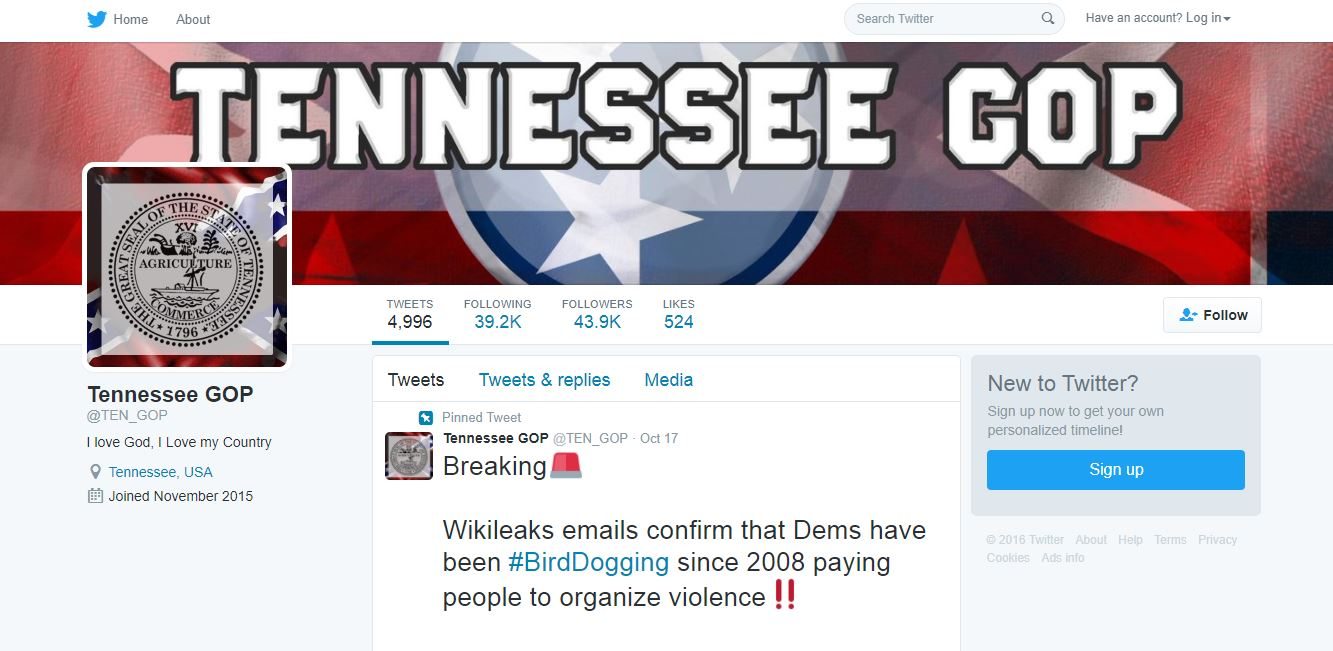
\includegraphics[width=11cm]{Ten_GOP.jpeg}
    \caption{@TEN\_GOP, Russian Troll Account}
    \label{fig:Russian Troll Account @TEN_GOP}
\end{figure} which is mentioned repeatedly in the Mueller report and claimed to be the official twitter of the Tennessee Republican Party. It racked up over 100,000 followers and frequently shared false information regarding voter fraud which was then retweeted by multiple individuals key to the Trump campaign, such as Donald Trump Jr., Eric Trump, Kellyanne Conway, Brad Parscale, and retired General Michael Flynn. As will be discussed later in the section on partisanship, individuals will conform to the opinions of the rest of a group, even if it runs contrary to their personal convictions or facts they've personally observed \cite{asch1956studies}, especially in politically charged environments \cite{bullock2007experiments,housholder2014facebook}. In this case, since the misinformation was being amplified and effectively cosigned by key political figures, rank-and-file Republicans believed @TEN\_GOP's fraud. This is the heart of the ethical objection: while incendiary opinions and statements may evoke strong polarized responses, 
the viral spread of misinformation intends, at its core, to exploit human weakness, gaslight its recipients, and rob them of the freedom to make informed decisions.


\subsubsection{Humanitarian Objection to Fake News}
The humanitarian arguments are the most important reasons for curbing the spread of disinformation. In previous sections, the "pizzagate" story where a person brought an AR-15 into a restaurant was discussed, but this is far from a unique example. Hours after the 2013 Boston Marathon Bombing, members of social media hypothesized that an innocent Brown University student was behind the attack \cite{starbird2014rumors}; he committed suicide shortly after. A father of a child who was killed during the 2012 Sandy Hook shooting was harassed by social media members convinced that the shooting was a hoax \cite{williamson2019alex}; he too committed suicide shortly after. On September 9th 2020, a conspiracy theory began that the fires in Oregon were started by the left-wing activist group called Antifa \cite{robinson2020oregon}; on September 11th, the FBI put out a statement declaring the reports untrue \cite{fbi2020portland}; on September 12th, Facebook began removing these untrue posts; weeks later, Oregon officials were still wasting resources that should have been going towards firefighting to handle the non-stop deluge of calls and emails about the rumor \cite{wilson2020oregon}. Most recently, on January 6th, 2021, incited by the former President of the United States's debunked claims over election fraud and a baseless internet conspiracy called Q-Anon, a mob broke into the U.S. Capitol and threatened to execute members of Congress and the Vice President \cite{fandos2021trump}; five people were killed directly from riot \cite{Levenson2021capitol}.

Not all misinformation leads to active cases of violence. Misinformation exacerbated the Ebola epidemic in West Africa \cite{shultz2016role}, interfered with measles vaccination efforts \cite{hussain2018anti}, and disrupted health policies and procedures during the current COVID-19 pandemic \cite{bagherpour2020covid,world2020novel,zarocostas2020fight,depoux2020pandemic,habersaat2020ten,van2020using}. Groups that were fed misinformation that downplayed the severity of COVID-19 saw a higher lack of compliance with safety measures -- such as mask wearing and social distancing -- and a higher number of cases and deaths \cite{bursztyn2020misinformation}. Even though the United States has seen numerous days of more than 4,000 deaths due to the virus, only half of the country is currently planning on getting a vaccine when it's available \cite{cornwall2020just}. The misinformation content has run the gamut from misleading messages about the actions or policies of public officials \cite{brennen2020types}, to suggesting the vaccine is a conduit for Bill Gates to inject microchips into people \cite{sanders2020difference}, to blaming 5G cell towers \cite{jolley2020pylons,goodman2020coronavirus}, to inciting people to vandalism \cite{spring2020coronavirus}, to, in some cases, promoting mob violence and mass poisonings \cite{depoux2020pandemic}. Even if the final violent example is stripped away, the potentially unchecked spread of deadly disease is cause enough for concern. 

\subsubsection{Summary}
To summarize, misinformation is not protected by the First Amendment, is ethically wrong, and can have life-or-death consequences. This thesis does not seek to root out every misstatement, ill-thought out opinion, or dubious political attack ad. Instead, it is only focused on content that could provide a clear threat to election integrity, human life, etc. This limited scope is fundamentally different from the approaches taken by other recent literature on the topic, and will be discussed further there.

\subsection{Fake News Definition}
Before continuing, it's important to get a clear definition of what is meant by the term "fake news". The primary and most frequently cited definition of fake news comes from Allcott \& Gentzkow: "[they are] articles that are intentionally and verifiably false, and could mislead readers" \cite{allcott2017social}. Several existing studies adopt this definition \cite{conroy2015automatic,klein2017fake,rubin2015deception,rubin2017deception,mustafaraj2017fake,potthast2017stylometric}, and most attempt to parse out the further differences between \textit{misinformation}, \textit{disinformation}, \textit{rumor}, \textit{fake news}, etc. \cite{zimdars2020fake,  difonzo2007rumor,flynn2017nature,garrett2013undermining,wu2016mining}. Wu et al. provide the following diagram of their proposed parsing:
 \begin{figure}[htp]
    \centering
    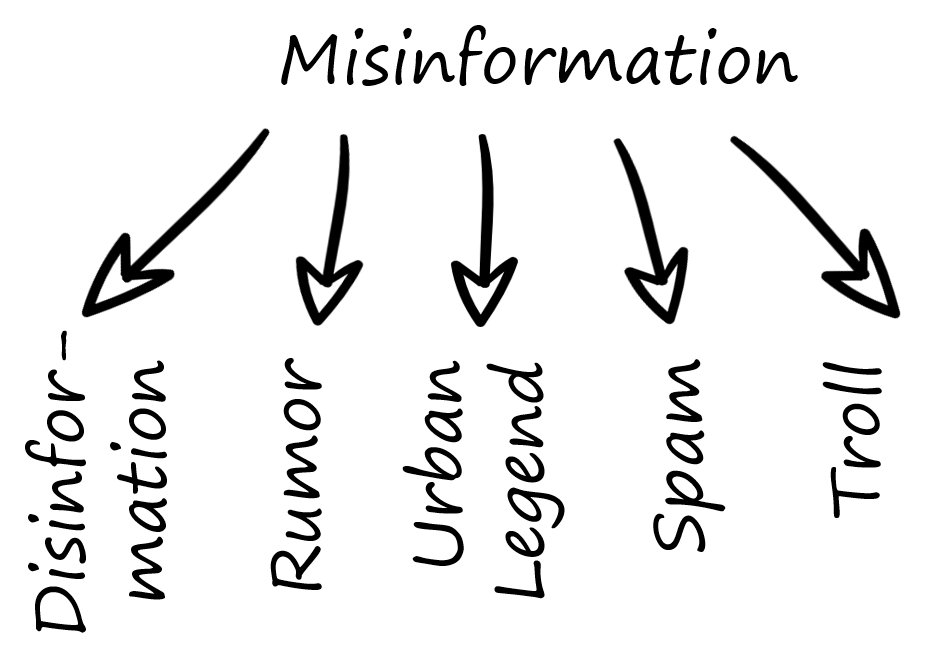
\includegraphics[width=4cm]{misinformation graphic.png}
    \caption{Misinformation Labels \cite{wu2016mining}}
    \label{fig:misinformation graphic.png}
\end{figure}


The dividing line between most of these categories is the level of intentionality: e.g. \textit{misinformation} is false but the creator has no verifiable  intent to mislead the reader, whereas \textit{disinformation} is false and the creator has a high intent to mislead the reader, and \textit{rumors} may be true or false, but the truth value is currently undetermined.

This has lead to an alternative definition from Klein \& Wueller: "[misinformation is] a news article that is intentionally and verifiably false". \cite{klein2017fake}. This definition has seen growth and has also been accepted by current studies \cite{shu2017fake, liu2018early}.

To bridge this gap, a more epistemological approach is proposed. For every tweet $t$ in the set of tweets $T$, there is a corresponding truth value $\tau$ between 0 and 1 (0 means something is completely false and 1 means something is completely true):
\begin{equation}
\label{truthvalues}
    \forall \ t \in T \ \exists \ \tau, \tau \in \mathbb{R} \ | \ 0 \leq \tau \leq 1
\end{equation}
Several previous works on this topic set $\tau \in \ \{0,1\}$ \cite{liu2018early,shu2017fake}. This is incorrect, as statements may be false, partially true, mostly true, or completely true. For example, this tweet from conservative provocateur Charlie Kirk (fig. \ref{fig:Charlie Kirk Tweet, May 4, 2020})  \begin{figure}[h]
    \centering
    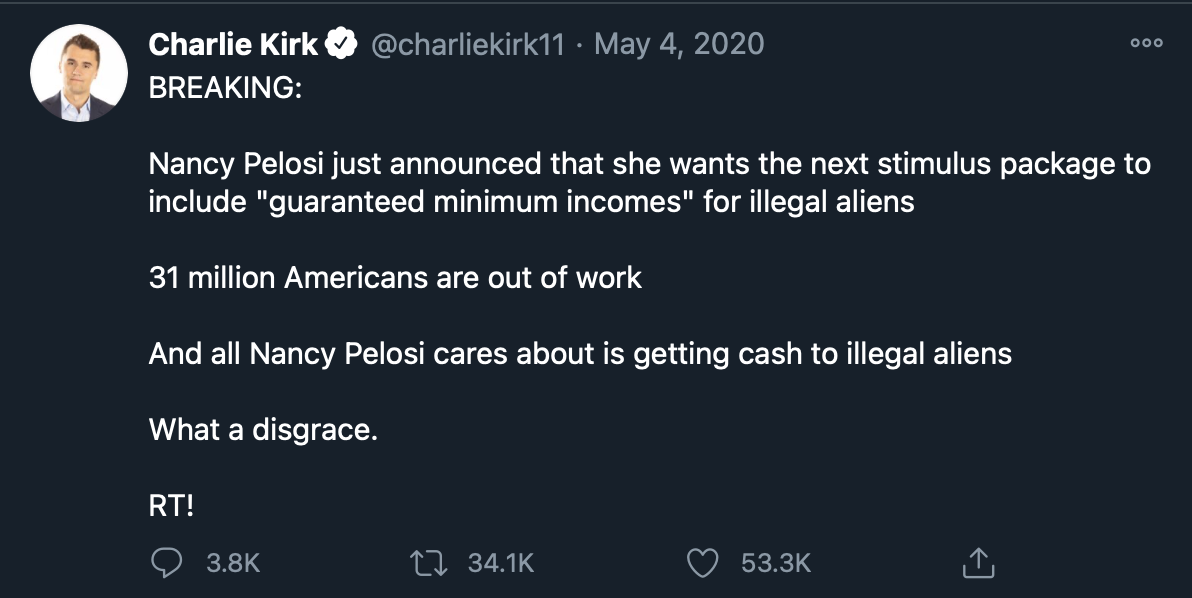
\includegraphics[width=11cm]{CharlieKirk Tweet.png}
    \caption{Charlie Kirk Tweet}
    \label{fig:Charlie Kirk Tweet, May 4, 2020}
\end{figure} was rated "mostly false" by Snopes \cite{lee2020pelosi}: while Speaker Pelosi did say in an interview that she wanted to consider "guaranteed incomes" for Americans, including foreign workers without social security numbers \cite{pelosi2020maher}, she did not clearly define if "guaranteed income" meant the 2020 Paycheck Protection Plan (PPP) or something more akin to Universal Basic Income (UBI) as Kirk implies; she requested congress "consider it" and did not says she "wanted it"; both PPP and UBI would have directly affected \textit{all of} the 31 million Americans out of work rather than \textit{only} the undocumented immigrants as Kirk suggests. Therefore, since it is \textit{mostly} false but not \textit{completely} false, it would be unfair to say that $\tau_k = 0$ for this tweet; $ 0 < \tau_k < 0.5$ is more accurate. 


In another example, this tweet from Bernie Sanders is "mostly true" (fig. \ref{fig:Bernie Sanders Tweet, Oct 13, 2020}). 
 \begin{figure}[h]
    \centering
    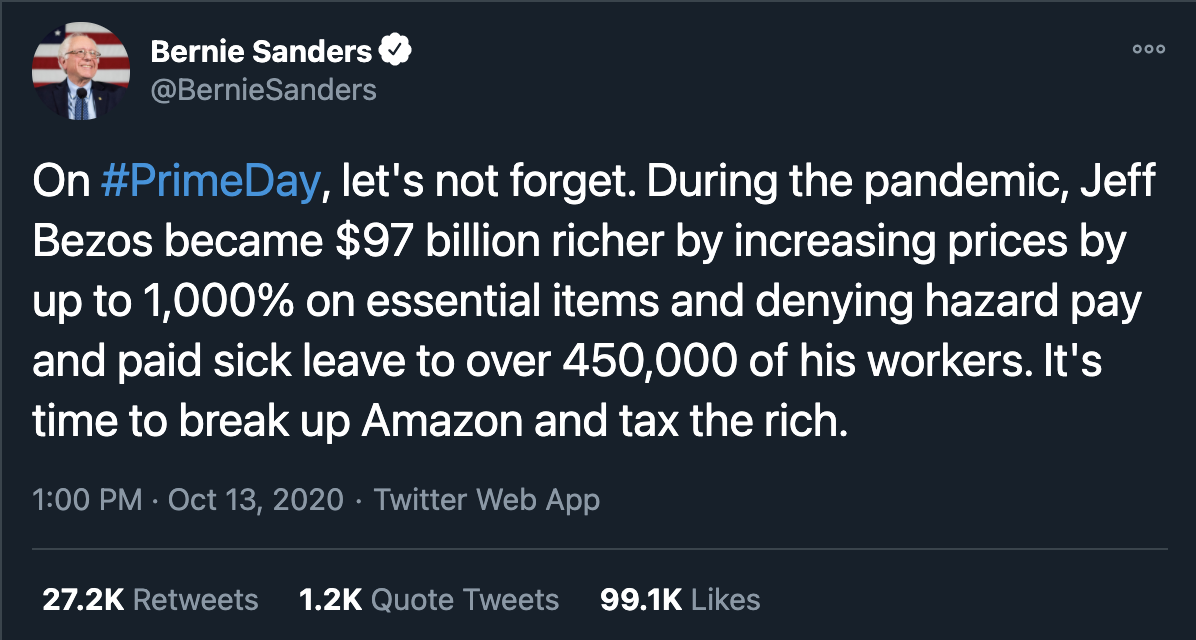
\includegraphics[width=11cm]{BernieTweet.png}
    \caption{Bernie Sanders Tweet}
    \label{fig:Bernie Sanders Tweet, Oct 13, 2020}
\end{figure}
While it is true that Amazon's employees have been denied hazard or sick pay (or have struggled with the mostly automated Amazon HR) \cite{cnbc2020amazon,guardian2020amazon}, and Jeff Bezos's wealth increased by almost 80\% during 2020 due to Amazon's 40\% increase in sales year over year for Q2 (and the majority of his wealth is tied to Amazon shares) \cite{Stebbins2020bezos}, other articles discussing the increase in price on essential items point out that this was mostly Amazon \textbf{re-sellers} using the Amazon marketplace, not Amazon directly \cite{nicas2020sanitizer, kim2020price,gibson2020amazon}, Amazon banned over 6,000 of these price gougers \cite{bezos2020letter}, and that in cases where Amazon's price-generating AI had raised the price to an extreme level, it was returned to a reasonable level before Sen. Sanders wrote this tweet \cite{harman2020prime}. Therefore, it would not be reasonable to say that $\tau_s = 1$ for this tweet; it is $ 0.5 < \tau_s < 1$. 

Both Charlie Kirk's tweet and Senator Sanders's tweet fall under the purview of this thesis based on section \ref{Problem Statement}: each of them is trying to influence a political discussion and uses statements that are not entirely true to persuade susceptible readers. At the same time, they are not equivalent. Charlie Kirk's tweet featured a single true sentence and many surrounding falsehoods, while Senator Sanders's tweet had many true statements and one untrue (or at least misleading) statement. Much like how it was unreasonable to say $\tau_k = 0$ or $\tau_s = 1$, it is also unreasonable to say $\tau_k = \tau_s$. This nuance is meaningful and is not captured in the other literature. Therefore, an alternative solution to determining truth values must be used.

In \underline{Critique of Pure Reason}, Immanuel Kant proposed that statements should be broken into four groups: \textit{analytic a priori}, \textit{analytic a posteriori}, \textit{synthetic a priori}, and \textit{synthetic a posteriori} \cite{kant1908critique,frege1988collected,quine1951main}. \textit{Analytic} statements, per Kant, have the predicate contained in the subject, whereas \textit{synthetic} statements require a combination of understandings; \textit{a priori} statements are known without needing experience, whereas \textit{a posteriori} statements require experience to know if they are true \cite{wright1997companion}. 

A discussion on the four groups of statements, examples, and analysis are in appendix \ref{truthvalue appendix}, but, to summarize here, this thesis will only cover \textit{synthetic a posteriori} statements for which a truth value has not been determined. It will also cover statements that could be hyperbole, sarcasm, or irony (Appendix \ref{hyperbole}), as a random user may not immediately recognize that the content they are reading is sarcastic. It also does not differentiate between intentional and unintentional false statements. The question of intentionality is appropriate when determining punishment or if actions reach the level of fraud (and are therefore worthy of legal action), but it is not relevant to this thesis. A rapidly spreading false tweet about election fraud is equally destructive regardless of malicious intent.

It is important not to separate rumor from misinformation as Wu et al. or DiFonzo \& Bordia do since rumors can be just as destructive. In the section on the Humanitarian cause for this problem, examples were given regarding people who had committed suicide after being the victims of rumors \cite{starbird2014rumors,williamson2019alex}. The rumor that Antifa started the fires in Oregon hurt the firefighting efforts in the region  \cite{robinson2020oregon}. Baseless accusations of voter fraud led to five deaths in a riot at the capitol and the impeachment of a former US President \cite{fandos2021trump,Levenson2021capitol}.  Wu et al. and DiFonzo \& Bordia would have called all of these "rumors" up until they were officially debunked, yet this delineation did not stop them from having very deadly and serious consequences in the interim.

It also important to separate out hate speech, spam, and scientific misinformation from generalized misinformation (Table \ref{tab:misinformationexamples} in appendix \ref{truthvalueappendixsummary}). These are tasks that current machine learning is uniquely suited for, already have a great deal of available literature \cite{xu2019exploiting,wang2010detecting,ahmed2018detecting,al2019spam,oriola2020evaluating,gaydhani2018detecting,al2020lies,farrell2019evidence}, and which this thesis does not plan to improve upon. By narrowing this thesis's scope and using these other tools in an auxiliary fashion, this thesis can focus on curbing the viral spread of misinformation that is currently being insufficiently defended against. 



\section{Literature Review}
In all of the literature reviewed for this thesis on the topic fake news, there was very little if any time spent discussing the currently implemented solutions and their shortcomings. This thesis will try to rectify that and show why alternative solutions are needed in comparison to the status quo.

After this, there will be a brief analysis of other relevant literature and why they fall short of solving the problem.

\subsection{Currently Implemented Solutions}
This section will look at Facebook's current solution, as it is more robust than Twitter's. Twitter currently only allows for flagging of political misinformation that is directly related to a political event, census, or impersonation (fig \ref{img:TwitterPolitics}):
\begin{figure}[htp]
    \centering
    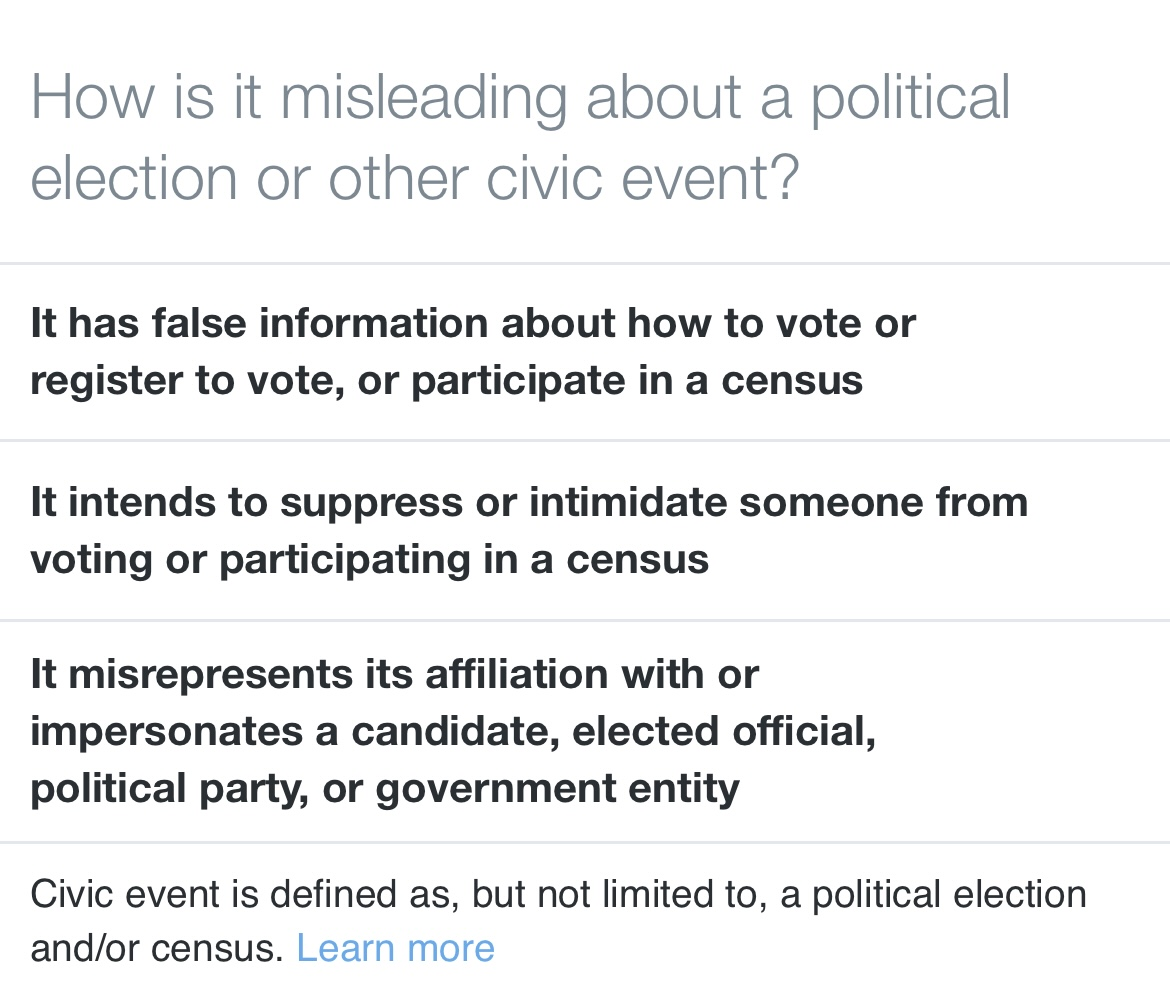
\includegraphics[width=6cm]{TwitterPolitics.jpg}
    \caption{Options for Flagging a Misleading Political Post on Twitter, Dec 2020}
    \label{img:TwitterPolitics}
\end{figure}

In his 2018 testimony to congress, Mark Zuckerberg stated that Facebook's processes with content reviewers had room for improvement, saying \begin{quote}"... unfortunately, with the amount of content in our systems and the current systems that we have in place to review, we make a relatively small percent of mistakes in content review but that is too many, and this is an area where we need to improve..." \cite{energy2018facebook}\end{quote} and then pivoted to discussing the need for AI solutions, given the need for scalibility.

In his 2020 testimony to congress, Zuckerberg stated that they had tripled the security team to 35,000 employees, that they're funding new security technologies to prevent emerging fake threats such as "deep fakes", and that they have implemented resource centers for hot button topics like COVID-19 and the 2020 election \cite{zuckerberg2020}.


As of this thesis, Facebook currently has a preemptive solution and a two-step solution:
\renewcommand{\labelenumii}{\Roman{enumii}}
\begin{itemize}
\item The preemptive solution is to add a “context” button to all political posts, which a user can click on for more information \cite{smith2018designing}.
 \item If a post has been shared and is untrue, the following two-step solution is used:
 \begin{enumerate}
     \item It requires an outside individual to report the post. 
     \item After the post is reported, then it is  sent to 3rd-party fact checkers for verification. 
     \begin{itemize}
     \item Third party fact checkers must log in to the Facebook dashboard and then provide a link proving the story is false (they cannot simply mark a story as untrue).
     \end{itemize}
 \end{enumerate}
 \end{itemize}
 
 In Facebook’s case, after they have determined a particular post is false, then the post is shown less frequently (80 percent less), other posts of the same link or image will also be shown less, it will be unable to be converted into an ad later, and someone re-sharing this post will be given a notification that the information is likely false \cite{owen2016clamping,facebook2020fact}.
 
 The punishment for routine offenders or for routine fake stories that point to a common domain is a loss of advertising rights and a loss of ability to monetize \cite{facebook2020fact}.
 
 %%%%%% 
 \subsection{Current Literature Alternative Solutions}
 
 
 
 \subsection{Issues with Solutions Discussion in Section 2.1 and 2.2}
 \subsubsection{Issues with Preemptive Solution}
 The "context" button is ineffective for several reasons. 
 
 First, it assumes that people will actively search for context when viewing a link. People are unlikely to feel the need to do further research if they agree with or believe the headline as presented \cite{nyhan2010corrections}. This problem is augmented by the fact that headlines are often misleading and written to draw the strongest possible emotional response \cite{chesney2017incongruent,ecker2014effects,bell1984good,molek2013towards,kilgo2018new,vettehen2008explaining}. For example with the \textit{Express} newspaper from the UK (from Ecker, et al.):
 \begin{itemize}
 \item Headline: Air pollution now leading cause of lung cancer
\item Evidence within article: “We now know that outdoor air pollution is not only a major risk to health in general, but also a leading \textbf{environmental} cause of cancer deaths.” Dr. Kurt Straif, of IARC [emphasis added]
 \end{itemize}
 
 Or from the \textit{Independent}'s Facebook page \cite{chesney2017incongruent}:
 \begin{itemize}
\item Social media post copy: Enjoy it while you
can
\item Social media headline \footnotetext[1]{https://www.facebook.com/TheIndependentOn-line/posts/10154972799736636}\footnotemark[1]: Scientists have predicted the end of sex
\item Article headline\footnotemark[2]\footnotetext[2]{Will Worley (2016): http://www.independent.co.uk/news/science/sex-unnecessary-designer-babies-stanfordprofessor-says-a6957636.html}: Sex will be made unnecessary by ‘designer babies’, professor says
\item Evidence within article: Professor Henry Greely believes that in as little as 20 years, most children will be conceived in a laboratory, rather than through sexual intercourse.
 \end{itemize}
 
 While there have been attempts to track down misleading headlines, they have primarily centered around \textit{click-bait} or tabloid headlines \cite{chen2015misleading,chakraborty2016stop} that require the user to click to find out the information, i.e. "Here’s What Happens When You Put A Few Little Kids In A Room With 2 Dolls In 2 Different Colors" \cite{chen2015misleading}. While this will help with some problems, both the \textit{Express} and \textit{The Independent} articles would not be caught by the proposed algorithms. 
 
 
Given that only 59\% of all shared URLs are ever clicked on Twitter \cite{gabielkov2016social} and there is clear evidence of misleading headlines, Twitter added in a feature that prompts users to read articles rather than just headlines before sharing the article \cite{reuters2020article}. Unsurprisingly, the backlash was immediate (fig: \ref{fig:House Judiciary GOP Tweet}):
 \begin{figure}[htp]
    \centering
    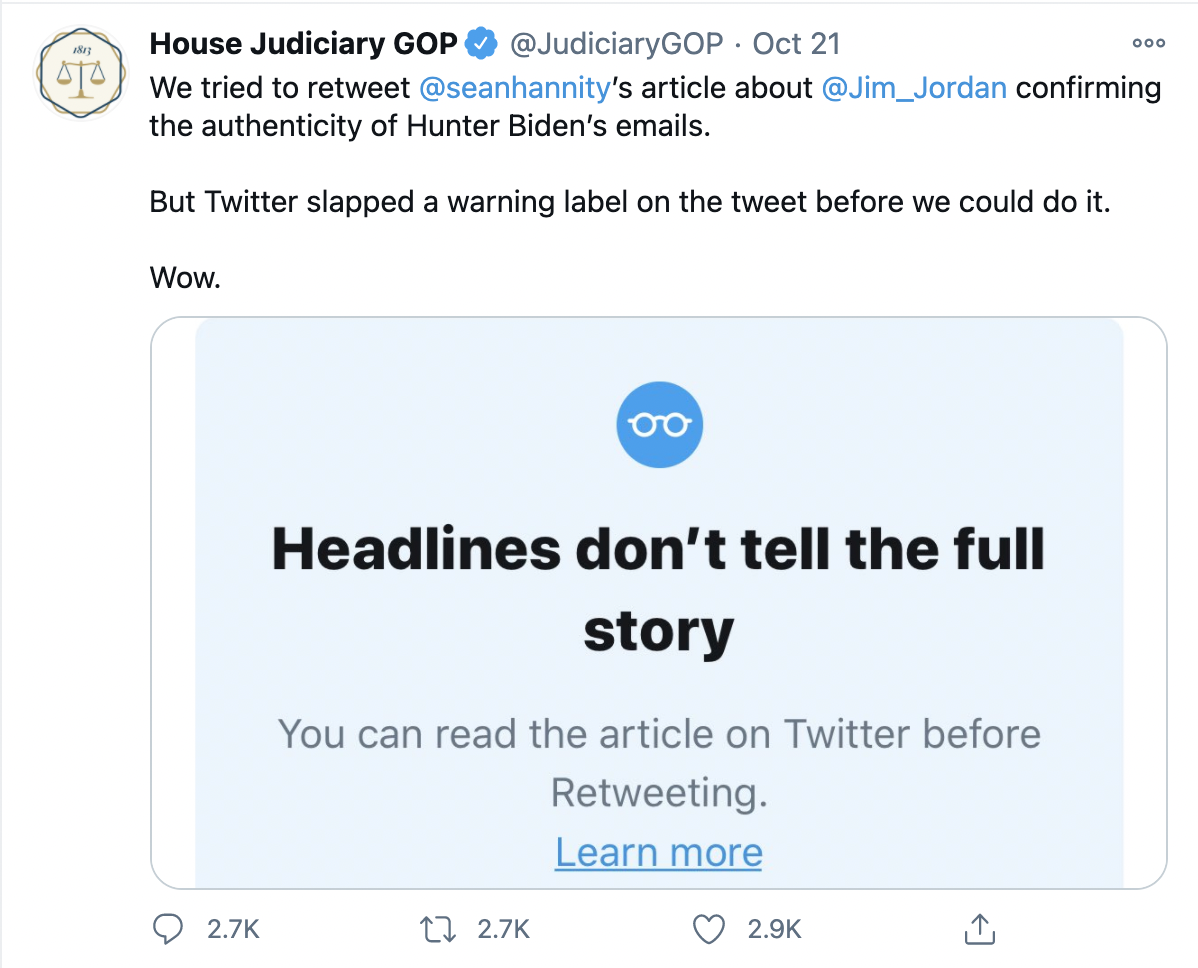
\includegraphics[width=8cm]{JudiciaryTweet.png}
    \caption{House Judiciary GOP Tweet}
    \label{fig:House Judiciary GOP Tweet}
\end{figure}

As will be discussed shortly, this fits the problem of \textit{echo chambers} wherein the primary question is not "is this correct" but "does it align with the views of my network?" 

To summarize, the proposed preemptive solution is ineffective because:
\begin{itemize}
\item 41\% of the time, someone will retweet an article without having read more than the headline. \cite{gabielkov2016social}
\item Headlines are written to be intentionally misleading, or at least to generate a strong emotional response from the reader.\cite{chesney2017incongruent}
\item Readers are unlikely to fact-check, question, or feel compelled to do outside research on an article if the have a strong emotional response to it.\cite{nyhan2010corrections}
\item Blanket warnings without explanation are likely to generate backlash \cite{reuters2020article}
 
 \end{itemize}

\subsubsection{Issues With the Two-Step Solution: Echo Chambers}
\label{sec: echo chambers}
 The key first step for the two-step solution is that an individual must report the post as false. This requires a level of self policing that it is unlikely given the prevalence of \textit{echo chambers}. 
 
Because social media seeks to connect like minded individuals, it has a tendency to generate \textit{echo chambers}, or closed networks with high repetition of content and low diversity of thought \cite{adibi2005proceedings, bastian2009international, pariser2011filter,bozdag2015breaking}. While not every closed homogeneous network is inherently bad -- they can operate as self-help groups \cite{kast2012under} or can encourage positive behavior like reducing prejudice \cite{paluck2011peer} -- there is a clear and well documented history that people are influenced by others in their network \cite{cialdini2004social,bollinger2012peer, bond201261,gerber2008social,gerber2009descriptive,meer2011brother,paluck2012salience,del2016spreading,bessi2015viral} and this can be destructive in the context of misinformation. For this paper's purposes, partisanship $\rho$, is defined as being on a scale of 0 to 1 with 0 being extremely left-wing and 1 being extremely right wing (a normalized version of most one-dimensional scales of the topic). Therefore, for all users $u$ in the sets of users $U$:
\begin{equation}
\label{basepartisanship}
    \forall \ u \in U \ \exists \ \rho \in \mathbb{R} \ | \ 0 \leq \rho \leq 1
\end{equation}
From here, $\rho_k$, the partisan leaning of some unique user $u_k$ is directly proportional to the average partisan leaning of the \textit{echo chamber} network $n_n$ (here and elsewhere, a network, $n$, is defined as the total set of "neighbors" or other nodes that the user is connected to either by following or being followed by) and can be described as follows:
 \begin{equation}
    \label{ech chamber}
        \langle \rho_n \rangle = \frac{1}{|n_n|}\sum_{i=1}^{|n_n|}{\rho_i}, (u_i \in n_n, n_n \in N)
 \end{equation}
 \begin{equation}
    \label{leaningproportionaltonetwork}
        \rho_k \sim \langle \rho_n \rangle
 \end{equation}
 
 For validation of this, in Asch's classic experiment, he found that individuals will conform to the opinions of the rest of the group, even if it runs contrary to their personal convictions \cite{asch1956studies}. For a more recent political example, in Bullock's experiments he found that participants would change their opinions on a particular topic if they were told that the party they identify with held an opposing view, even if it was counter-intuitive, such as a Republican being told that the Republican party was against a conservative initiative \cite{bullock2007experiments}. Other research provides similar results: Republicans and Democrats are likely to accept a statement as being true and not feel the need to research personally if it comes from a preferred politician \cite{housholder2014facebook}; even if a preferred politician's statements are disproved, there is no shift in voting intentions, party identification, or overall perceived credibility of that politician \cite{swire2017processing}. 
 
This provides a perfect opening for malicious actors, as they are primarily focused on sharing and inflaming hyper-partisan and extreme views \cite{bastos2019brexit,hegelich2016social,mueller2019mueller}, such that the partisanship of a malicious actor, \textit{m}, from the set of malicious actors, \textit{M}, will be extreme: 
\begin{equation}
\label{trollpartisanship}
\forall \ m \in M, \exists \ \rho \in \{0,1\}.
\end{equation}

Mirroring viral spread seen in other scale-free network analyses \cite{pastor2001epidemic,cohen2003efficient}, this problem quickly escalates: as the number of malicious actors in the network, $|M| \in n$, increases, the group partisanship will shift towards the \{0,1\} binary, as can be seen by combining equations \ref{trollpartisanship} and \ref{ech chamber}: 
\begin{equation}
\langle \rho \rangle \rightarrow \rho_m \in \{0,1\}
\end{equation} 
And given Bullock's experiments and equation \ref{leaningproportionaltonetwork}:
\begin{equation}
\label{peopletoextremes}
    \forall u \in n: \rho \sim \langle \rho_n \rangle: \rho \rightarrow \rho_m
\end{equation}
Equation \ref{peopletoextremes} correlates perfectly with the social experiments by Asch and Bullock mentioned previously, and more recent research has confirmed these findings \cite{colliander2019fake,edelson2011following}. Even when the groups were anonymous users on the internet, users will still be motivated by a desire to conform to the group's opinions and will, if necessary, relinquish their own previous beliefs to fit in \cite{williams2000cyberostracism,zhu2012switch,tsikerdekis2013effects,breitsohl2015groupthink,winter2015they,hamilton2017s}. 

The closer $\langle \rho \rangle$ gets to 0 or 1, the more closed the network becomes, and the more resistant to fact-checking or corrective information coming from outside of their network \cite{garrett2013undermining,lord1979biased,edwards1996disconfirmation,redlawsk2002hot, taber2006motivated}. This explains both why even the release of President Obama's long form birth certificate only briefly subdued the conspiracy that he was not born in the United States \cite{nyhan2012new} and why the Pizzagate conspiracy discussed earlier lived even after it had been disproved months earlier -- so long as the corrective information came from outside of the echo-chamber, it was fundamentally dismissed.


\subsubsection{Partisanship} 
There is substantial research that Americans who identify as right-wing have historically been more susceptible than other subsets of the American population to fake news \cite{guess2019less,benkler2018network,grinberg2019fake,allcott2017social,badawy2018analyzing}, but more thorough analysis suggests that this pattern may not hold up moving forward.

First, there may be an over representation in terms of conservative vs. left misinformation in the analyzed data sets. In the Russian troll data set provided by Twitter, there were twice as many right leaning trolls as left leaning trolls \cite{freelon2020black,badawy2018analyzing,benkler2018network}. It is likely that this is a positive feedback loop: since conservatives were more likely to consume fake news, there were more trolls creating fake content for them, which they in turn would be more likely to share \cite{bakir2018fake,bodo2019interested,silverman2016analysis,pariser2011filter}. 


Second, a better predictor of willingness to share misinformation is general distrust in the media rather than political leaning \cite{hopp2020people,shin2017partisan,kahan2012ideology,lewandowsky2016motivated,swire2017processing,mourao2019fake}. This is further born out by the Russian "troll farm" known as the Internet Research Agency (IRA) heavily targeting two groups they determined were unlikely to trust the main stream media: far right-wing Americans and Black Americans \cite{diresta2019tactics,howard2019ira,boatwright2018troll,jamieson2020cyberwar,mueller2019mueller,freelon2020black}. In fact, the IRA spent a disproportionately high amount in micro-targeting Black Americans and generated a high return on their investment (the average misinformation post targeted at a Black American was 2.5 times more likely to receive an engagement, such as a like or retweet, from a real user than a misinformation post targeted at a general conservative American) \cite{howard2019ira,freelon2020black}.

Third, many harers of misinformation are more focused on empathy with a particular group \cite{winter2015they,rheault2016measuring,dale2017nlp} or engaging in signaling theory with a group \cite{connelly2011signaling,lampe2007familiar,spence2002signaling} rather than objective truth. Dominic Cummings callously stated while creating inaccurate content for the Leave campaign for Brexit that "accuracy is for snake-oil pussies" \cite{crace2016accuracy}, yet his point is widespread and in line with the analysis of \textit{echo chambers} in section \ref{sec: echo chambers}: in hyper-partisan situations, strongly held opinions that are counter to widely accepted narratives are seen primarily as signals of commonality \cite{yla2018populist,noppari2019user,lazer2018science,yla2019politicization,wasilewski2019us,freelon2020russian}. 


Fourth, there is no difference in propensity to share non-partisan misinformation, such as the dangers of living near power lines, the side-effects of MMR vaccines, or the safety of nuclear power reactors between people of various beliefs \cite{kahan2015climate,hara2016co,kahan2012ideology,lewandowsky2016motivated,barbera2015tweeting}.

Finally, most of the studies referenced previously looked at data from 2015/2016 and before. Since 2015, there has been a well documented global rise in populism on the left end of the spectrum to match the rise on the right that had previously existed and was documented earlier. For example, there was a 33x increase in membership in far-left organizations such as the Democratic Socialists of America between 2015 and 2020 \cite{godfrey2020thousands}, left-leaning populist groups in France saw outsized social media volume in the 2017 elections \cite{donadio2017french}, and the U.K's Labour party took a shift to the populist left under the leadership of Jeremy Corbyn starting in 2015 \cite{wainwright2018remarkable,hobson_fielding_2019}. 

This polarized shift can be statistically seen in the United States Congress by comparing the voting patterns of the 115th (Jan 2017 - Jan 2019) (fig. \ref{fig:115th House}) and 116th (Jan 2019 - Jan 2020) (fig. \ref{fig:116th House}) House of Representatives \cite{fivethirtyeight2018tracking}. In both of these illustrations, Democrats are blue, Republicans are red, Independents are orange, and the scale for each Representative is the same $0\leq \rho \leq 1$ scale seen in equation \ref{basepartisanship}. Here, a representative who always voted in line with President Trump's position (if he gave one on a particular bill) has $\rho = 1$, and someone who never voted in line with President Trump has $\rho = 0$:

 \begin{figure}[h]
\minipage{0.5\textwidth}
  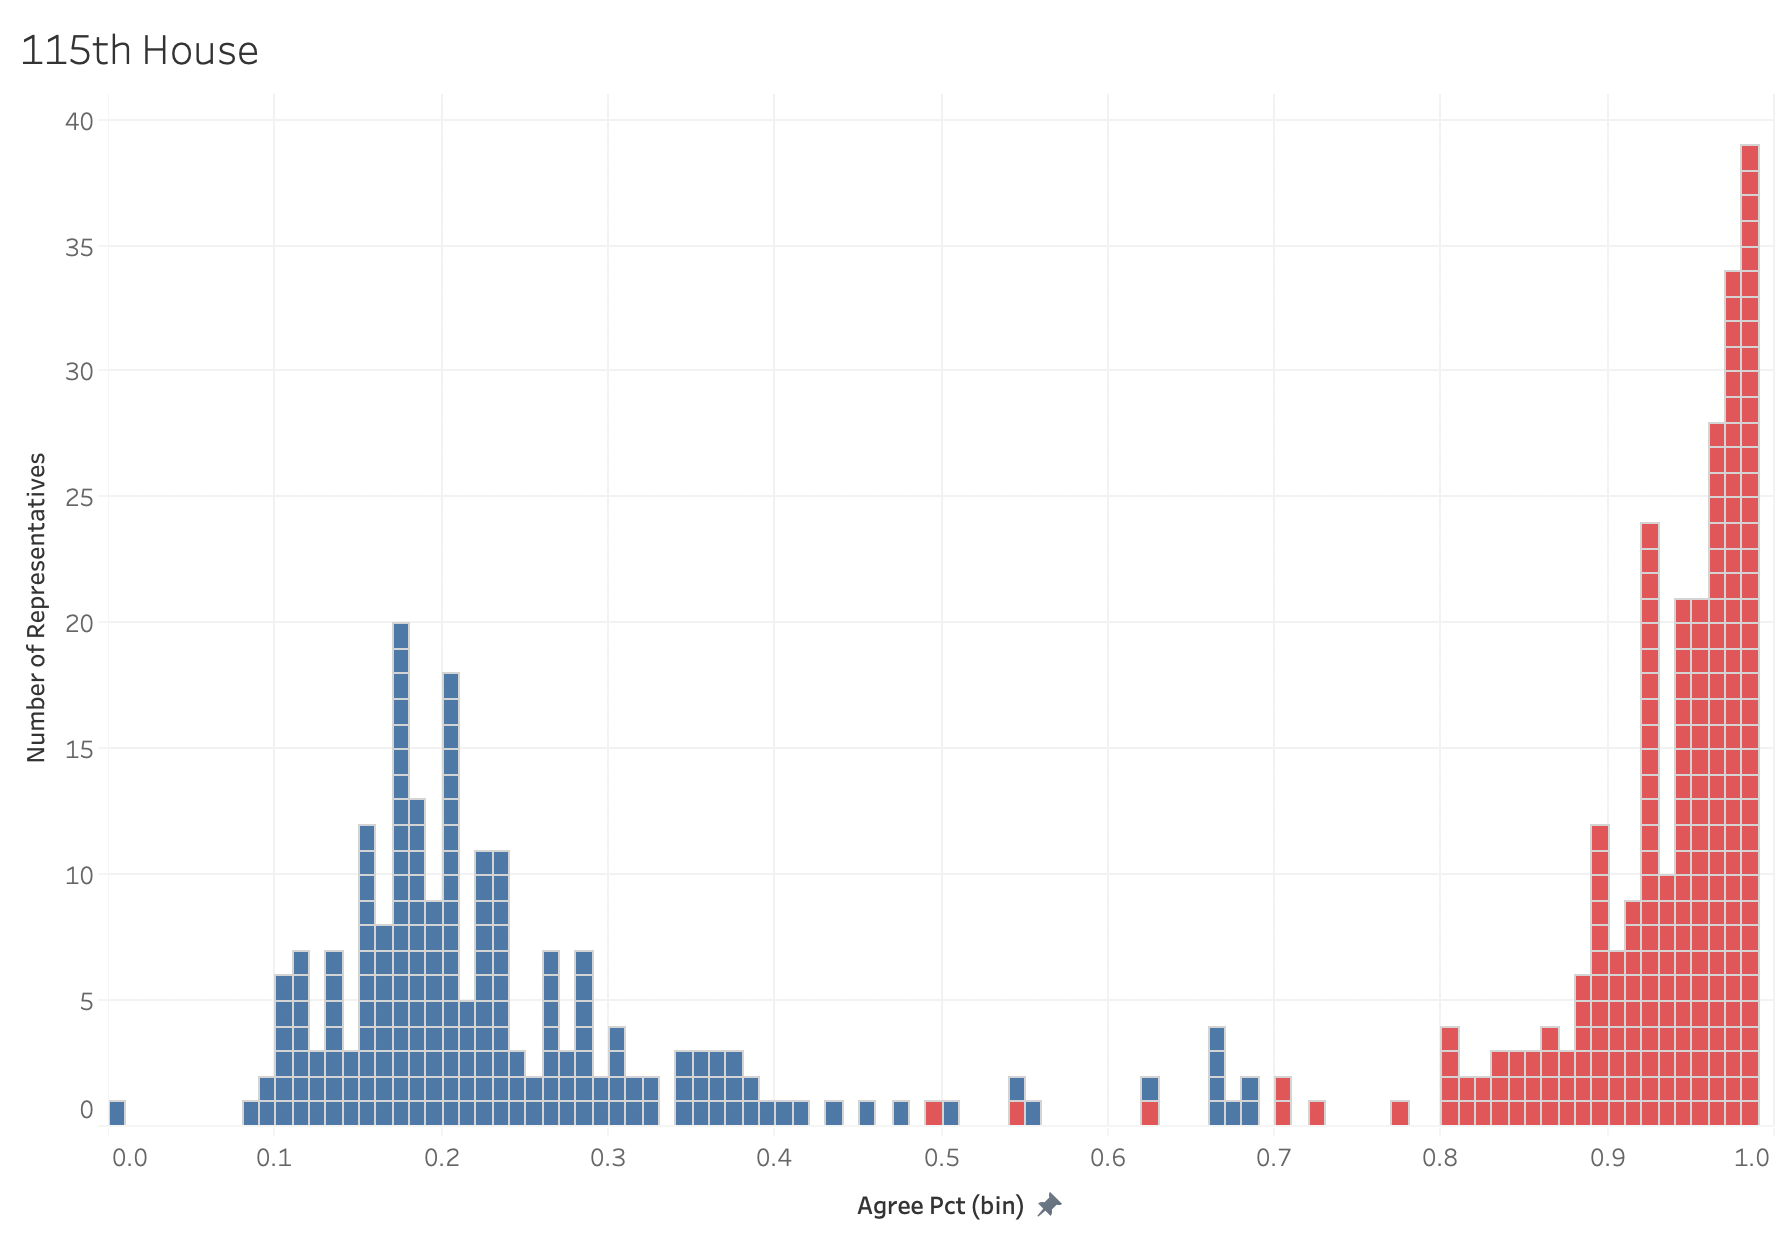
\includegraphics[width=\linewidth]{115th House.png}
  \caption{115th House of Representatives}\label{fig:115th House}
\endminipage\hfill
\minipage{0.5\textwidth}
  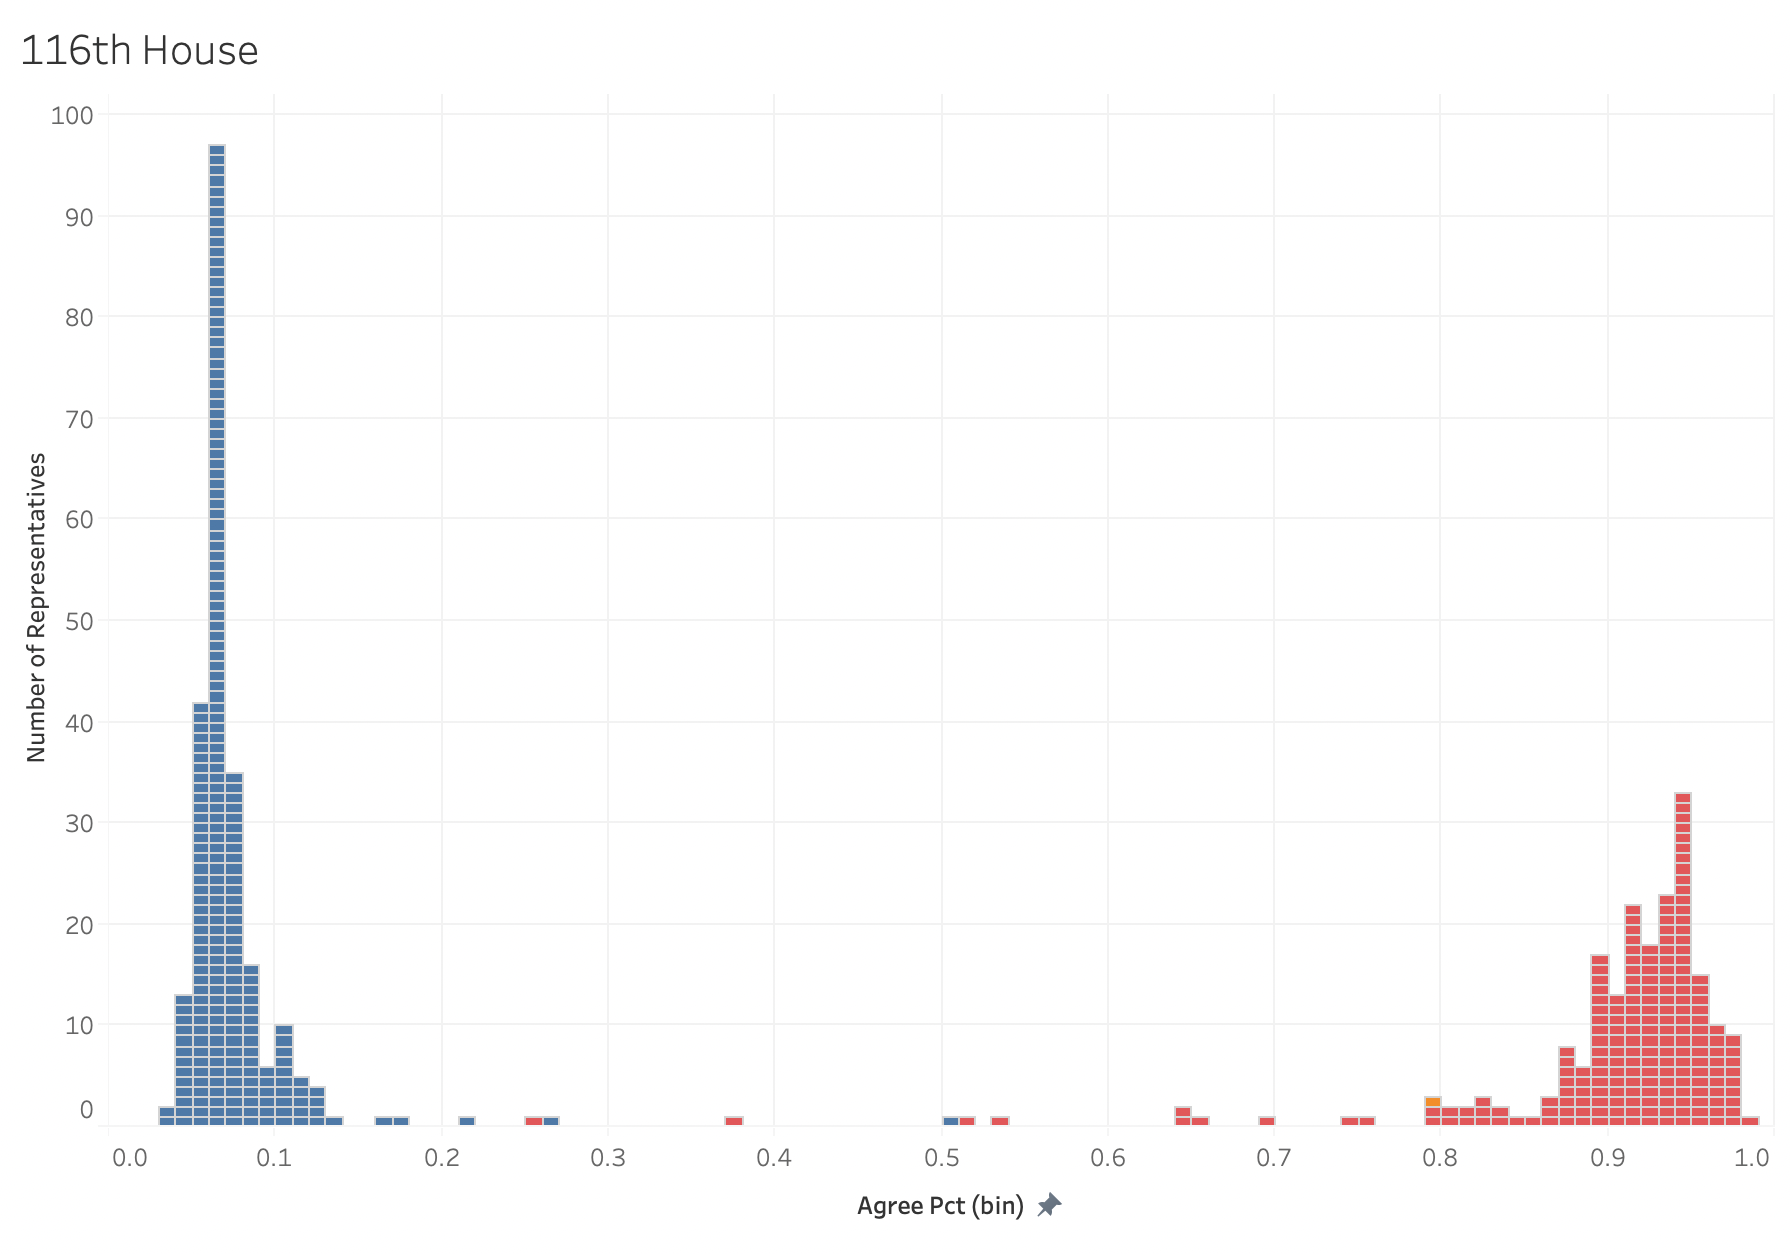
\includegraphics[width=\linewidth]{116th House.png}
  \caption{116th House of Representatives}\label{fig:116th House}
\endminipage\hfill
\end{figure}
 
 In the 115th congress, Republican members had an average $\langle \rho_r \rangle = 0.93$ and Democratic members had an average $\langle \rho_d \rangle = 0.24$. In the 116th congress, Republican members had an average $\langle \rho_r \rangle = 0.91$, Democratic members had an average $\langle \rho_d \rangle = 0.08$, and Independent members had an average $\langle \rho_i \rangle = 0.79$. While the Democratic party did pick up +40 seats in the 2018 midterms, simply adding or subtracting members does not imply a shift in partisanship as the Republican partisanship barely changed between the 115th and 116th Congress. For the state of Pennsylvania, which very narrowly broke for President Trump in 2016, the Democratic members had a $\langle \rho \rangle = 0.39$ in the 115th Congress and a $\langle \rho \rangle= 0.07$ in the 116th.
 
 For comparison, the US Senate is somewhat more stable, possibly because Senators are only up for election every 6 years instead of every 2, so turnover is less frequent. In the 115th congress, Republican senators had an average $\langle \rho_r \rangle = 0.91$, Democratic senators had an average $\langle \rho_d \rangle = 0.30$, and Independent senators had an average $\langle \rho_i \rangle = 0.30$. In the 116th congress, Republican senators had an average $\langle \rho_r \rangle = 0.83$, Democratic senators had an average $\langle \rho_d \rangle = 0.19$, and Independent senators had an average $\langle \rho_i \rangle = 0.22$.
 
 As illustrated before, a shift in the average partisanship of the network towards the \{0,1\} binary strongly correlates to populism and a susceptibility to misinformation \cite{hopp2020people,kahan2012ideology,mourao2019fake,shin2017partisan,swire2017processing,vargo2018agenda}. This can already been seen anecdotally, as there has been an uptick in left-leaning misinformation (or hyper-partisan opinions counter to the general accepted facts, per point two of this section)  since 2018, including information around a confrontation between MAGA-hat wearing teenagers, Black Israelites, and a Native American elder at the Lincoln Memorial in 2019 \cite{sacks2019maga,healy2019believing,pond2020complexity}, and the death of Breonna Taylor in 2020 \cite{duvall2020fact,kim2020fact}. 

 \subsubsection{Third Party Fact Checkers}
 The usage of third party fact checkers has two fundamental issues.
 
 First, there is a large volume of research over decades that ideologues on either side of the political spectrum will view the exact same content as being biased against them \cite{arpan2003experimental,baum2008eye,christen2002hostile,gunther2001predicting,gunther2004mapping,baum2004issue,gussin2004eye,lee2005liberal,vallone1985hostile}. This extends to fact-checking, as groups on both the left and the right post about claims of censorship when their content is removed or their reach is reduced \cite{Dreyfuss2020Now,Post2020Facebook,Millhiser2018Facebook}. 
 
 As Shin and Thorson note, however, closed networks are eager to fact check members who are not of their group. In 2018, Think Progress (a liberal Facebook fact checker) had an article on the Brett Kavanaugh Supreme Court confirmation hearing that was flagged as false by The Weekly Standard (a conservative Facebook fact checker) \cite{owen2018with}. Think Progress stated that then-Judge Kavanaugh had said during his hearing that he would kill Roe v. Wade \cite{millhiser2018brett}, a claim that was deemed false by the Weekly Standard and by FactCheck.org, a non-partisan fact-checking organization \cite{gore2018kavanaugh}. The Weekly Standard offered to remove its flag if Think Progress replaced the word "said" in the headline, as Judge Kavanaugh had not explicitly said that he would overturn Roe v. Wade. Think Progress argued that secondary and tertiary definitions of "said" made their headline correct, and instead accused Facebook of bias and censorship \cite{legum2018tweet}. Shortly after, several other liberal journalists made the same argument of censorship with none touching on whether or not the word "said" was truthful \cite{froomkin2018tweet,grim2018tweet,beutler2018tweet}. 
 
 This example matches the previous analysis of strongly held partisan views being "truer" than objective truth. It also aligns with other research that shows that closed groups are more than eager to fact-check individuals who do not belong to their group, such as Republicans fact checking Democrats and vice-versa \cite{shin2017partisan,iyengar2015fear}, and that they are unable or unwilling to recognize potential mischaracterizations of opposing viewpoints \cite{pennycook2019lazy,vargo2018agenda}. 
 
A better solution, clearly, would be only to use high quality non-partisan fact checkers, as they would be able to rise above the echo chamber issues. However, these well-regarded apolitical fact checkers, such as Snopes and the Associated Press, have either left their fact checking partnership with Facebook or stopped actively working. They argue that Facebook's process is manual, time consuming, ineffective, and does not provide adequate compensation for the time required to do the job thoroughly \cite{green2019message,coldeway2019update}. An ideal solution, then, most be one which limits the amount of time-consuming manual work, hence Zuckerberg's initial comments about AI being the key to solving this problem.

\subsubsection{Issues with Punishment}
By this point, it should be clear that the punishments imposed by Facebook are not effective, as they only seek to limit ad revenue and the ability to monetize. This implies a financial incentive for purveyors of incorrect information where, as has been shown, much of this is ideologically driven \cite{allcott2017social}. While these may be effective deterrents for the \textit{click-bait} or tabloid style headlines discussed earlier  \cite{chen2015misleading}, less than 0.1\% of traffic to fake news websites during the 2016 election came from paid media/advertising \cite{albright2016election2016}. 

The other key punishment that Facebook implements is on the actual post level. Posts deemed false are shown 80\% less frequently, and other posts showing the same link or image will also be shown less frequently. While this sounds promising, there is a fundamental flaw that can be exposed by examining Facebook's most recent papers on computer vision. Facebook's AI is a Convolutional Neural Network (CNN) \cite{carion2020end}, which is very good for detecting something in common across several images, such as a person's face \cite{kalinovskii2015compact}, but is easily fooled by changing parts of the image, such as adjusting font and colors, cropping, adding filters, etc \cite{sumbaly2020using}.

For example, this shutterstock image of Donald Trump (fig. \ref{fig:Trump Shutterstock Image}): 
 \begin{figure}[htp]
    \centering
    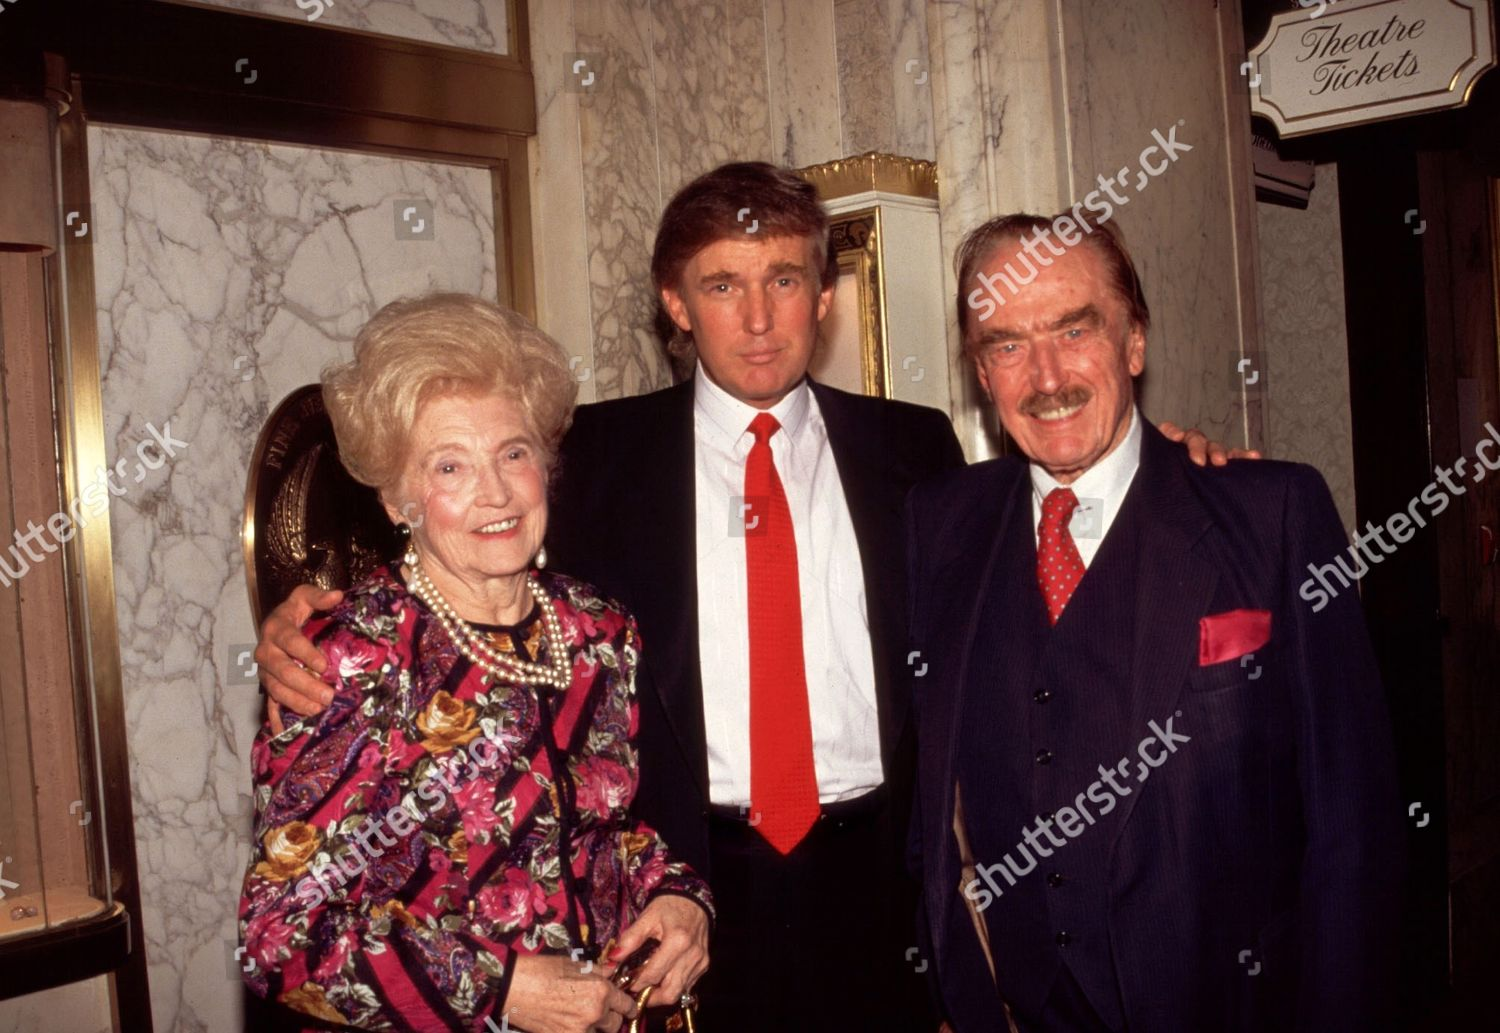
\includegraphics[width=8cm]{trumpkkk0.jpg}
    \caption{Trump Shutterstock Image}
    \label{fig:Trump Shutterstock Image}
\end{figure}

was photoshopped to make it appear as though his parents were wearing KKK robes. Reuters provided three different examples of the image that were widely shared on social media \cite{reuters2020trump} (Figures \ref{fig:TrumpKKK1}, \ref{fig:TrumpKKK2}, \ref{fig:TrumpKKK3}).

 \begin{figure}[h]
\minipage{0.32\textwidth}
  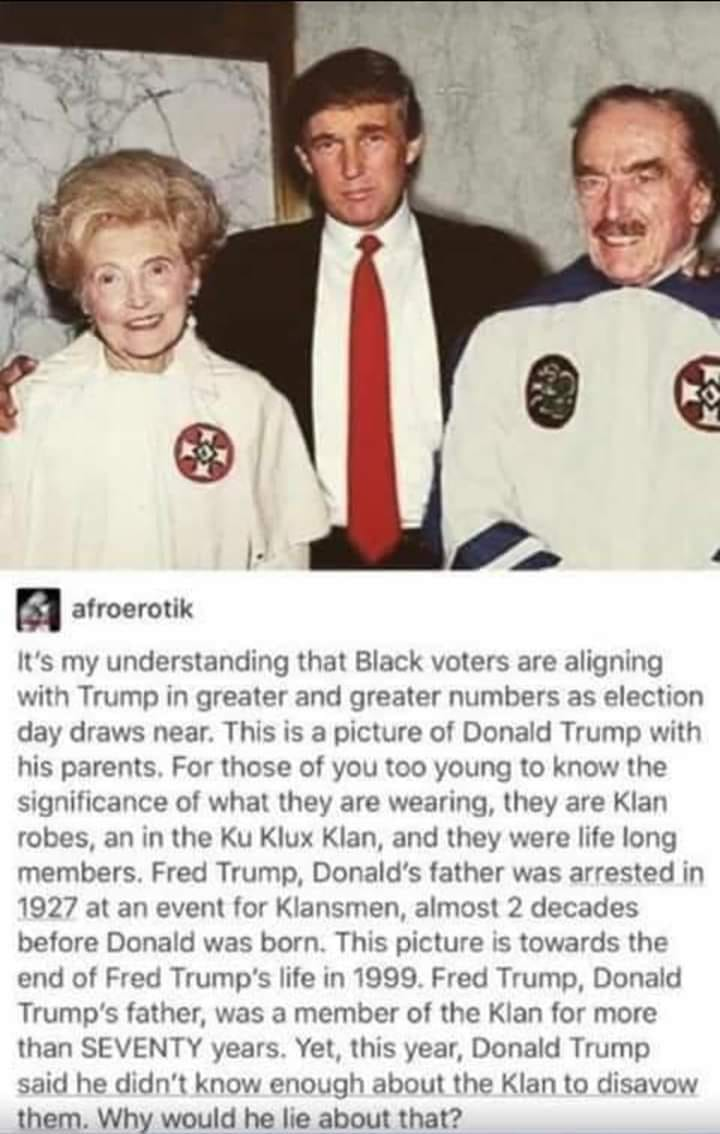
\includegraphics[width=\linewidth,height = 9cm]{trumpkkk1.jpg}
  \caption{Version 1 of Edited Trump Image}\label{fig:TrumpKKK1}
\endminipage\hfill
\minipage{0.32\textwidth}
  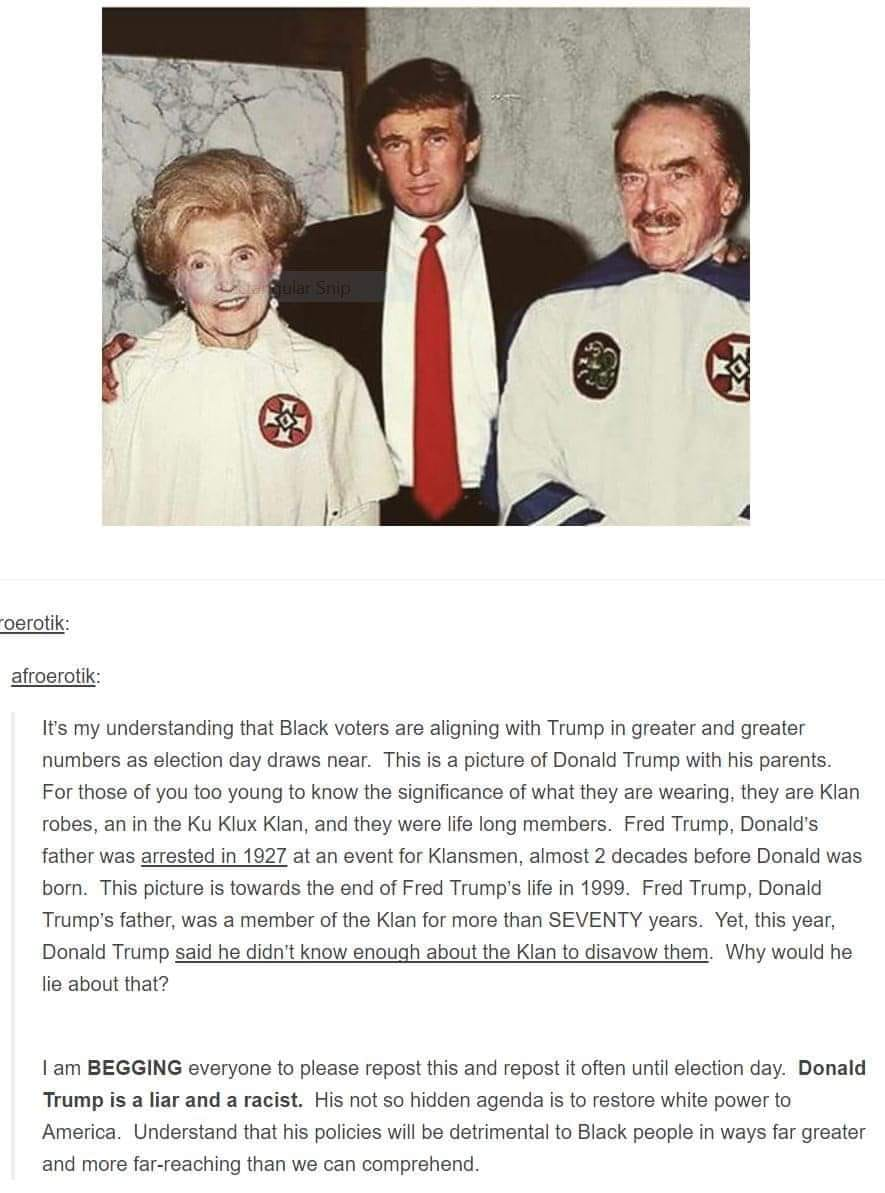
\includegraphics[width=\linewidth,height = 9cm]{trumpkkk2.jpg}
  \caption{Version 2 of Edited Trump Image}\label{fig:TrumpKKK2}
\endminipage\hfill
\minipage{0.32\textwidth}%
  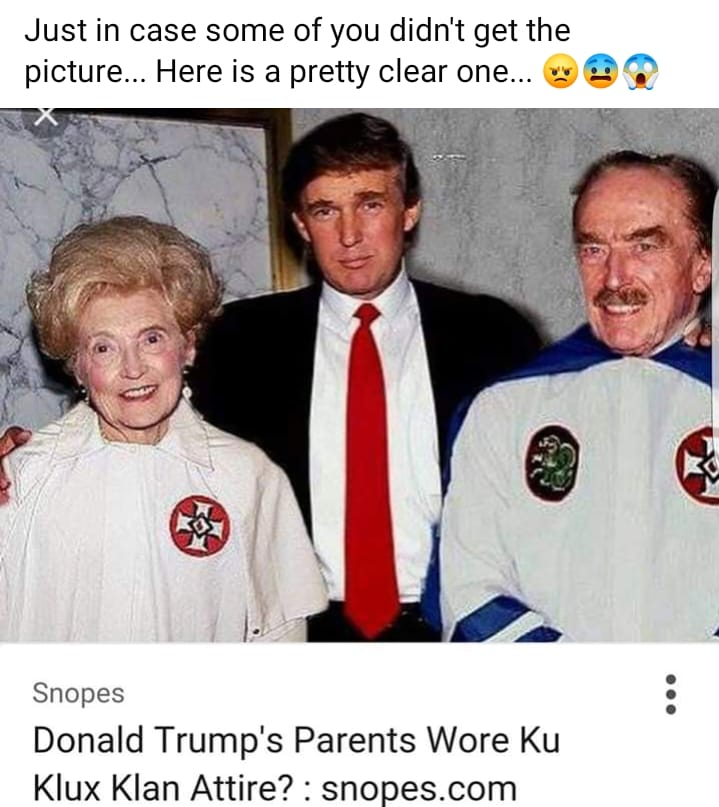
\includegraphics[width=\linewidth,height = 9cm]{trumpkkk3.jpg}
  \caption{Version 3 of Edited Trump Image}\label{fig:TrumpKKK3}
\endminipage
\end{figure}


To a human, all three of these images are roughly the same, but there is sufficient distorting in each image (e.g. some have removed pieces of the "shutterstock" watermark, others all of them; sections of the images have been cropped or stretched or mirrored; colors have been adjusted; etc.) combined with the variations in the text around the image to confuse a CNN. Facebook even admits that their CNN struggles to tell the difference between near-identical images and that there could be "thousands or millions of copies" of these undetected near-duplicates of already flagged content \cite{sumbaly2020using}. Their new solution, "SimSearchNet", is built specifically to solve this issue, but it is not fully effective yet. Avaaz, an activist organization with a focus on stopping the spread of fake news, found that 42\% of the misinformation content they analyzed in October was currently circumventing Facebook's policies. Even more disheartening, they were able to identify 738 posts that were not labeled as fake, in spite of having already been debunked, and had collectively racked up 5.6M interactions and 142M views \cite{schott2020brief}.

Some of these had the potential to influence the 2020 election, in spite of the extra measures Facebook and Twitter added \cite{dean2020facebook}: "While Facebook applied a contextual label to one false claim on a purple background about extra postage being required for mail-in ballots, another identical claim ran against a blue background with no intervention from Facebook. The former received 14,000 shares; the latter received 20,000" \cite{Fung2020facebook}.

Ultimately, neither of the proposed Facebook punishments are effective: reducing the ability to monetize is irrelevant for an ideological actor, and reducing the spread of an image or removing it entirely is insufficient if the same image can be recreated and re-shared so easily.

\subsubsection{Scale}
The issue of scale is not only non-trivial, but is unmentioned in the other literature on solving this issue. Attempting to crawl through every tweet and every URL posted would be an incredibly difficult task given that Facebook alone has 1.8 billion daily active users as of their Q3 2020 earnings report, with 2.54 billion daily active users of at least one tool in the Facebook portfolio (Facebook, Instagram, WhatsApp, etc.), with those numbers ballooning to 2.74 and 3.21 billion on a monthly level \cite{facebook2020q3}. Given that in 2014 Facebook generated 4 petabytes of data daily and ran 600,000 queries with 1 million map-reducing jobs when their total daily active users was 890 million \cite{bronson2015open}, a simple ratio would provide a conservative estimate that Facebook now generates at least 8.1 petabytes of data every day, with 1.2 million queries and 2.1 million map-reducing jobs. 

Many of the proposed solutions for fake news detection are RNN based, however RNNs are far too resource heavy to be successfully implemented at the necessary scale \cite{gehring2017novel, sze2017efficient}. Even transformer based attention models, like the ones suggested in the 2017 Facebook article on machine learning, require high amounts of compute power and primarily excel at tasks like language translation \cite{vaswani2017attention}. The detection of fake news is a more complex task, as a solution most not only decipher the language being used, but also interpret a representative truth value, and return a remove/don't-remove decision within a matter of hours of the initial post's timestamp, $p_i$.

As Facebook's digital footprint grows, a successful solution must be able to grow with it. 

\subsubsection{Summary}
To summarize, the current solution and issues are:
\renewcommand{\labelenumii}{\Roman{enumii}}
\begin{enumerate}
\item The preemptive solution is ineffective because users will not seek extra context
\begin{itemize}
\item Users will not seek extra context and will reject being prompted to look for extra context
\end{itemize}
\item An outside individual must report the post for further actions
 \begin{itemize}
     \item Users are unlikely to report posts that are in line with their partisan views
     \item Individual partisanship is strongly influenced by the beliefs of their network, which can be infiltrated by extremist ideology
     \item Extremist ideology on either side of the political spectrum is strongly resistant to fact checking, and maintaining beliefs that are opposed to generally accepted facts can actually be seen as proof of strong beliefs
    \end{itemize}
     \item After the post is reported, then it is  sent to 3rd-party fact checkers for verification. 
     \begin{itemize}
         \item Third party fact checkers are subject to the same biases as users
         \item There is no appeals process, so punitive flagging is possible
         \item Apolitical fact checkers are leaving or no longer active
     \end{itemize}
     \item Third party fact checkers must log in to the Facebook dashboard and then provide a link proving the story is false (they cannot simply mark a story as untrue).
     \begin{itemize}
         \item The process is manual and time consuming
         \item The payment from Facebook is insufficient for the time required to do the job correctly
     \end{itemize}
     \item Routine offender domains see decreased visibility, loss of advertising rights, and inability to monetize
     \begin{itemize}
         \item Loss of advertising rights is irrelevant to non-financially driven bad actors
         \item Decreased visibility (or removal) is easily circumvented by providing simple tweaks to the text or image
     \end{itemize}
 \end{enumerate}

\appendix
\section{Truth Values}
\label{truthvalue appendix}
\subsection{Analytic a Priori}
An \textit{analytic a priori} statement's truth value is "true by virtue of meanings and independent of fact" \cite{quine1951main}. 
For example, proposition 1: \begin{center}
    $P_1$: All triangles have three sides.
\end{center}
The predicate "having three sides" is contained within the meaning of the word "triangle". There is no need to observe a given triangle in order to know that it must have three sides.

For the purposes of this discussion, racial slurs and other such language shall be considered \textit{analytic a priori} hate speech, as there is no need to observe all racial slurs in order to know that they were created and used with hate speech as the intent. Hate speech are fundamentally false statements \cite{waldron2012harm}, which automatically mean $\tau = 0$ .

\subsection{Synthetic a Priori}
A \textit{synthetic a priori} statement is true if it is universally true, no experience is needed to confirm it, but it is also not definitional in nature:
\begin{center}
    $P_2$: The sum of two sides of a triangle are greater than the third side.
\end{center}
 
As with $P_1$, there is no need to measure every triangle in existence to confirm this statement is true, yet there is nothing contained in the definition of a triangle that implies this relationship between the three sides.

In this thesis, spam will be considered false \textit{synthetic a priori} statements. Naive-Bayes classifiers have been incredibly successful at detecting spam messages \cite{wang2010detecting,xu2019exploiting,ahmed2018detecting}, in large part because they consistently illustrate the same telltale signs of being spam: broken English, seemingly random URL links, etc. Therefore, \begin{center}
    $P_3$: Spam messages are unsolicited messages that feature broken English, random links, etc. \\
$P_4$: Unsolicited messages that meet the requirements of $P_3$ are not truthful.\\
$C$: Spam messages are not truthful.
\end{center}
 
This syllogism is logically valid even though there is nothing in the definition of the word "spam" that leads to a truth value. Therefor, spam messages may also be set to $\tau = 0$.


\subsection{Analytic a Posteriori}
A statement is \textit{analytic a posteriori} if it is true by virtue of its definition, but requires empirical evidence to discover it \cite{kripke1972naming}. Kripke gives the example of Venus being both the morning and evening star: \begin{center}
   $P_5$: Venus is the morning star.\\
$P_6$: Venus is the evening star.\\
$C$: The morning star is the evening star. 
\end{center}


While this statement is necessarily true based off of the definitions of "morning star" and "evening star", it can't be considered \textit{a priori} true, as Homer (12th century BCE) refers to the morning and evening stars as separate objects, and it isn't until Pythagoras (500 BCE) that it is a scientifically accepted fact that the morning and evening stars refer to the same object, Venus \cite{dunne1978voyage}.

Scientific information would largely fall into this category. Propositions such as: 
\begin{center}
    $P_7$: Water is H$_2$O.
\end{center} 
are necessarily true and definitionally true, but were not known since the start of time -- in the case of water, it was not formally known until Avogadro in 1811. Scientific conspiracies such as the Earth being flat, would therefore be examples of \textit{analytic a posteriori} misinformation, as the Earth being round is scientifically true and definitionally true, per Frege, as any complete definition of the Earth would have to imply that it was a round planet \cite{frege2003sense}. Scientific misinformation that is definitionally true can also be set to $\tau = 0$.

\subsection{Synthetic a Posteriori}
A statement is \textit{synthetic a posteriori} if its truth value is contingent upon experience and non-definitional in nature. Statements such as: \begin{center}
    $P_8$: John Adams and Thomas Jefferson both died on July 4th, 1826.
\end{center}

would be \textit{synthetic a posteriori} true statements, as they are objectively true, but there is nothing in the definition of "John Adams" or "Thomas Jefferson" that implies a death date. External verification is necessary in order to determine the truthfulness of the statement.

The majority of the statements that Wu et al. attempt to break into subgroups would all be considered \textit{sythentic a posteriori} statements here: rumors, legends, etc. may or may not be true, but require external validation in order to determine their truthfulness.

\subsection{Hyperbole, Sarcasm, and Irony}
\label{hyperbole}
Finally, hyperbole, sarcasm, and irony should be separated from our truth value set, as these are statements that are intentionally false to point to a greater underlying truth. 
Current literature on using NLP to decipher sarcasm and irony primarily revolves around unexpected word combinations \cite{barbieri2014modelling,buschmeier2014impact,ghosh2015sarcastic} or RoBERTa recurrent neural networks \cite{potamias2020transformer}, and they all examine publicly available data sets, namely the Riloff Twitter set \cite{riloff2013sarcasm}, the Pt{\'a}{\v{c}}ek Twitter set \cite{ptavcek2014sarcasm}, the Khodak Reddit set \cite{khodak2017large} and two "Semantic Evaluation Workshop Tasks" \cite{van2018semeval,ghosh2015semeval}. Many of these are able to generate quite high F1 scores, especially the RCNN-RoBERTa transformer proposed by Potomias, Siolas, and Stafylopatis, whose F1 score was consistently around 0.8 in each of the unique data sets. 

However, as Oprea and Magdy point out, tools that are successful in one data set struggle in other data sets. Models trained in the Riloff data set can generate an F1 score above 0.8, but those same models will generate an F1 score near 0.5 (which is the same as random guessing) when applied to the Pt{\'a}{\v{c}}ek set \cite{oprea2019exploring}. This implies there are extreme differences in how groups express and perceive irony/sarcasm/hyperbole. Those differences are beyond the scope of what RNNs and RCNNs can currently successfully grasp. Therefore an alternative solution to handling irony on a global level is necessary.
\subsection{Summary}
\label{truthvalueappendixsummary}
To summarize, with examples of misinformation according to each distinction (table \ref{tab:misinformationexamples}),
\begin{table}[htbp]
    \centering
    \begin{tabular}{ |p{3cm}|p{5cm}|p{5cm}|}
    \hline
    & Analytic & Synthetic\\
    \hline
    A Priori & Hate Speech & Spam\\
    \hline
    A Posteriori &  Scientific Misinformation  & General Misinformation\\
    \hline
    \end{tabular}
    \caption{Misinformation Examples of Analytic/Synthetic Distinctions}
    \label{tab:misinformationexamples}
\end{table}
in terms of truth values, $\tau$, \textit{a priori} and \textit{analytic} statements are binary, but \textit{synthetic a posteriori} sentences may have a range of truthfulness (such as being misleading, partially true, mostly true, etc.) (table \ref{tab:truthvalues}).

\begin{table}[h!]
\centering
\begin{tabular}{ |p{3cm}|p{5cm}|p{5cm}|}
 \hline
  & Analytic & Synthetic\\
 \hline
 A Priori & $\tau \in\ \mathbb{B}$ & $\tau \in\ \mathbb{B}$\\
 \hline
 A Posteriori &  $\tau \in\ \mathbb{B}$  & $\tau \in \mathbb{R} \ | \ 0 \leq \tau \leq 1$ \\
 \hline
\end{tabular}
\caption{Truth Values of Analytic/Synthetic Distinctions}
\label{tab:truthvalues}
\end{table}

These proposed distinctions better capture the breadth of misinformation than the previously provided definitions: as with Klein, it concurs that intentionality is not relevant in determining truth value; unlike Wu et al. or DiFonzo \& Bordia, it makes no distinction between types of misinformation such as "rumor" and "misinformation"; unlike Liu \& Wu, it separates hate speech, spam, and scientific misinformation from generalized misinformation; unlike all other examples, it includes sarcasm, hyperbole, and irony. 



\section{Maths}
\newpage
%%%%%%%%%%%%%%%%%%%%%%%
%% The bibliography

\bibliographystyle{plain}
\bibliography{bibliography.bib}


\end{document}